\documentclass{article}
\usepackage[utf8]{inputenc}

\title{Advanced Programming Labwork 7}
\author{Tom HERBRETEAU }
\date{November 2018}

\usepackage{natbib}
\usepackage{graphicx}
\usepackage{pgfplots}
\pgfplotsset{compat=newest}

\begin{document}

\maketitle
Every performance measures are done on ICT4 with eiffel.jpg, without counting the image saving.
\section{Introduction}
We have to normalize the input image to extend grey level to [0;255]. To do this, we need to find the min and max grey of the input image, and then, apply a grayscale stretch.
\section{Implementation}
To implement it, I choose to use 4 kernels, the first one to extract a array of min/max between the first and second half of the input. Then I use two kernel to reduce the min/max to the minimum and the maximum, then I apply grayscale stretch.
To optimize I choose to use 3 kernels instead of 2, because I choose to work on array of Int instead of array of uchar3, so I need to convert it, and apply a first reduction by dividing by two the number of entries while creating the min and max tab.
Then I use a while loop who launch the reduceToMin kernel and the reduceToMax kernel. These kernel use REDUCE pattern to get the minimum/maximum value of a group of 1024 value (the blocksize actually). At each step, the loop divide by 2 the number of value, and we loop until there is less than 1024 value in global array.

\section{Result}
The process last 27.7ms to compute the stretched image. On eiffel.jpg, the output is the same because the image already have pixel going from 0 to 255.
\newline
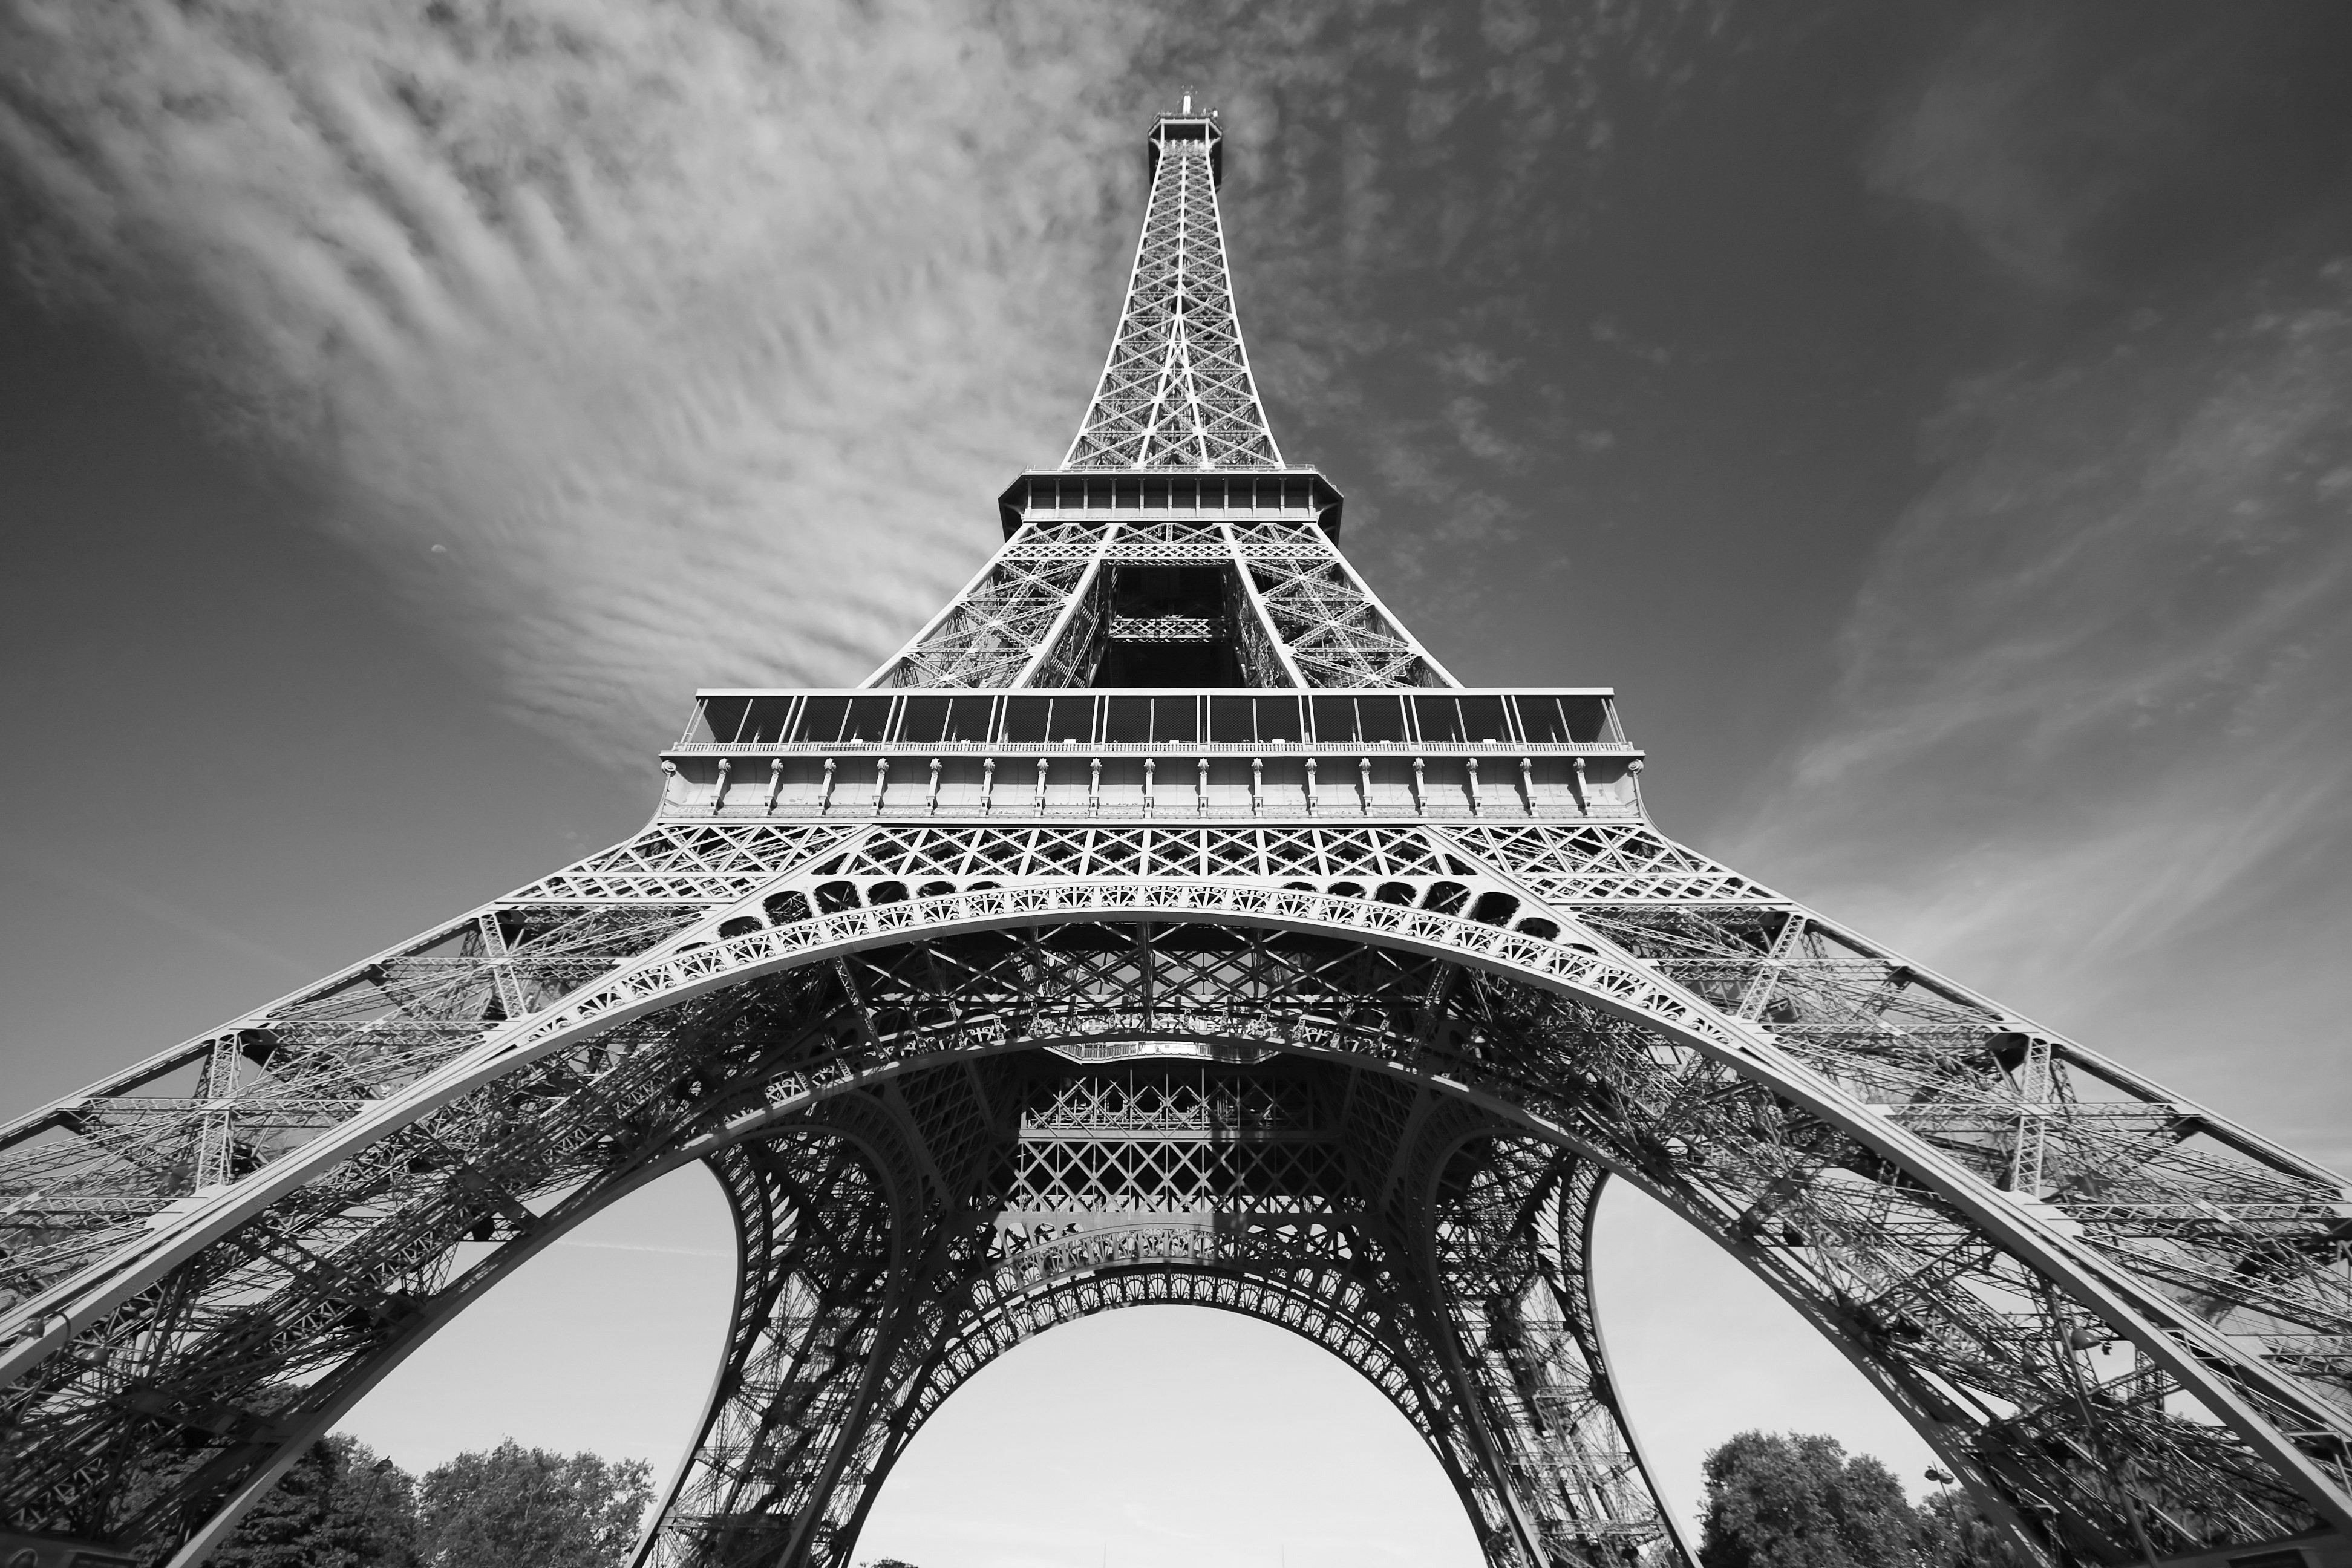
\includegraphics[width=\textwidth]{labwork7-gpu-out.jpg}
\bibliographystyle{plain}
\end{document}
